\documentclass[letterpaper,12pt,]{article}

\usepackage[%
    left=1in,%
    right=1in,%
    top=1in,%
    bottom=1.0in,%
    paperheight=11in,%
    paperwidth=8.5in%
]{geometry}%

\usepackage{listings}
\usepackage{graphicx}
\usepackage{amsmath}
\usepackage[font=small,skip=-2pt]{caption}
\usepackage{subcaption}
\usepackage{hyperref}
\usepackage{booktabs}
\usepackage{pdfpages}
\usepackage{pgffor}


\lstdefinestyle{mystyle}{
    %backgroundcolor=\color{backcolour},
    %commentstyle=\color{codegreen},
    %keywordstyle=\color{magenta},
    %numberstyle=\tiny\color{codegray},
    %stringstyle=\color{codepurple},
    basicstyle=\footnotesize,
    breakatwhitespace=false,
    breaklines=true,
    captionpos=b,
    keepspaces=true,
    numbers=left,
    numberstyle=\footnotesize,
    stepnumber=1,
    numbersep=5pt,
    showspaces=false,
    showstringspaces=false,
    showtabs=false,
    tabsize=2,
    frame=single
}
\lstset{frame=single}

\pagestyle{empty} % Remove page numbering
\linespread{1.5} % Line Spacing

\begin{document}

\begin{titlepage}

\newcommand{\HRule}{\rule{\linewidth}{0.5mm}} % Defines a new command for the horizontal lines, change thickness here

\center % Center everything on the page
 
%----------------------------------------------------------------------------------------
%	HEADING SECTIONS
%----------------------------------------------------------------------------------------


\textsc{\LARGE McGill University}\\[3.5cm]
\textsc{\Large Computational Aerodynamics}\\[0.5cm] 
\textsc{\large MECH 539}\\[2.5cm]

%----------------------------------------------------------------------------------------
%	TITLE SECTION
%----------------------------------------------------------------------------------------

{ \huge \bfseries Project 2}\\[1.5cm] % Title of your document

\HRule \\[0.4cm]
%----------------------------------------------------------------------------------------
%	AUTHOR SECTION
%----------------------------------------------------------------------------------------

\begin{minipage}{0.4\textwidth}
\begin{flushleft} \large
\emph{Name:}\\
Doug \textsc{Shi-Dong} % Your name
\end{flushleft}
\end{minipage}
~
\begin{minipage}{0.4\textwidth}
\begin{flushright} \large
\emph{Student ID:} \\
260466662\\
\end{flushright}
\end{minipage}\\[4cm]

\vfill{}
{\large February 18, 2016}\\[2cm]

\end{titlepage}



\section*{Grid}

The coarse grid has $80$ nodes in the $x$-direction and $40$ nodes in the $y$-direction with a constant spacing $dx = 0.025$ along the airfoil and $dy=0.025$ on the first layer in the $y$-direction.
The grid spans $x=[-0.05, 47.5]$ and $y=[0.0, 50.9]$.

When a finer grid is required, additional points are inserted evenly between each node to refine the grid.
The $159 \times 79$ and $317 \times 157$ grids will be refered as the medium and fine grids respectively.

\section*{Mach Number Study}

In this section, the coarse grid is used and the freestream Mach number $M_{in}$ is varied between $[0.80,0.90]$ with increments of $0.02$.
Figure \ref{fig:conv2} shows the convergence of the algorithm down to 5\textsc{E-}15.
Higher $M_{in}$ seem to take slightly more iterations to converge.
It can be explained by looking at the earlier iterations shown in Figure \ref{fig:conv22}.
The discontinuous jumps in residual are probably due to the sonic switches in the Murman-Cole algorithm turning on and off.
Higher $M_{in}$ (in the transonic region) will result in more inaccurate initial conditions and therefore, more turning on and off the switches.

The surface pressure coefficient is shown in Figure \ref{fig:cpsurf}.
As the $M_{in}$ increases, a shock forms and starts moving aft, until it reaches the trailing edge.
Moreover, the strength of the shock also increases since a higher decrease in static pressure is required to retrieve the atmosphere pressure.
Figure \ref{fig:cpcontour8084} and \ref{fig:cpcontour8690} show the coefficient of pressure contours for the different $M_{in}$.

\begin{figure}[!htbp]
    \centering
    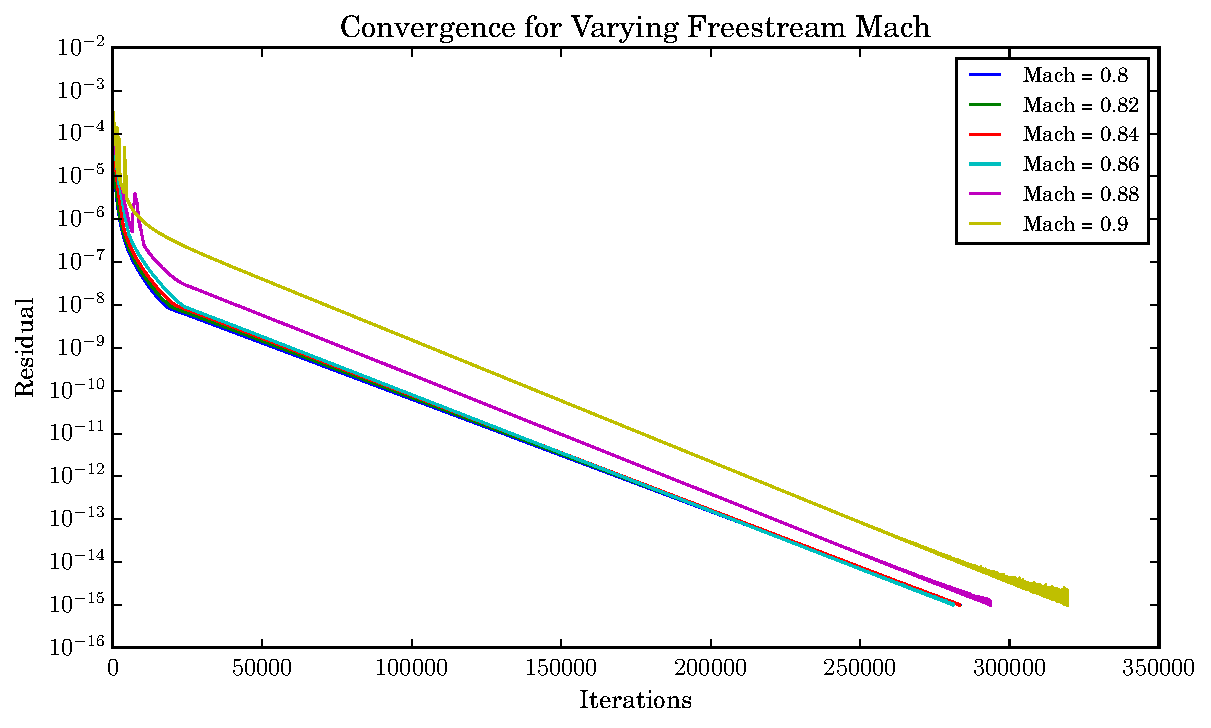
\includegraphics[width = 0.85\textwidth]{./Figures/convergenceq2.pdf}
    \caption {Convergence of Murman-Cole Algorithm using Gauss-Seidel}
    \label{fig:conv2}
\end{figure}

\begin{figure}[!htbp]
    \centering
    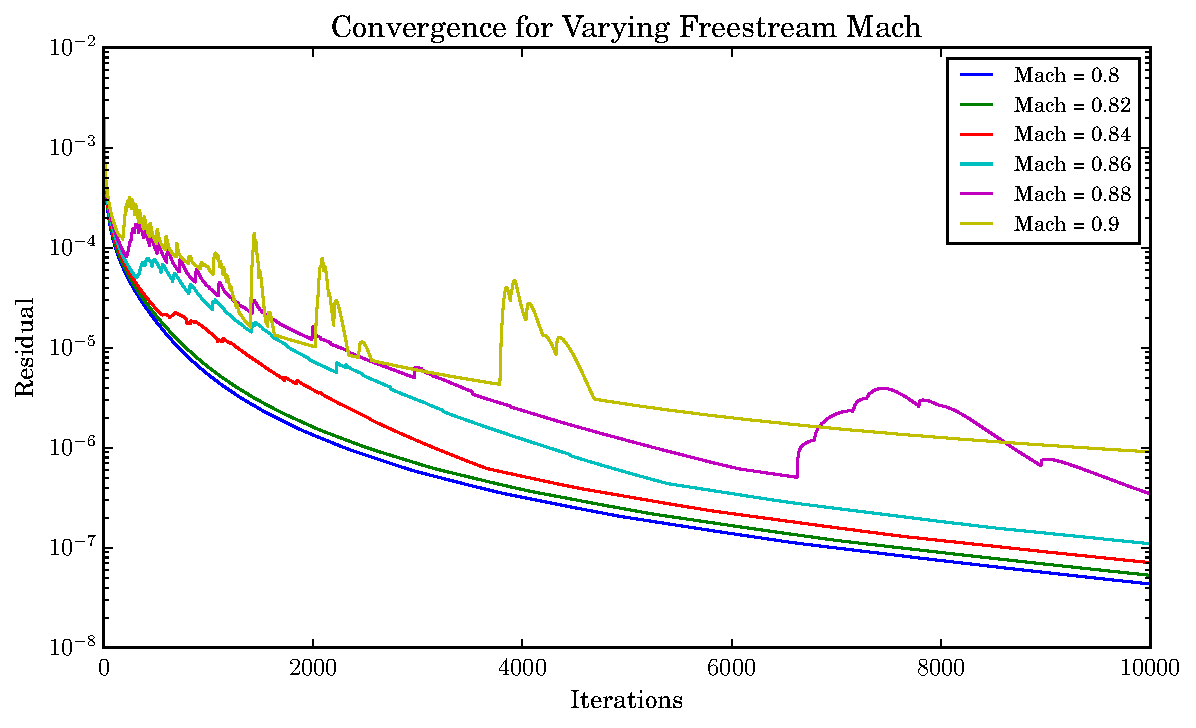
\includegraphics[width = 0.85\textwidth]{./Figures/convergenceq22.pdf}
    \caption{Earlier Convergence of Murman-Cole Algorithm using Gauss-Seidel}
    \label{fig:conv22}
\end{figure}

\begin{figure}[!htbp]
    \centering
    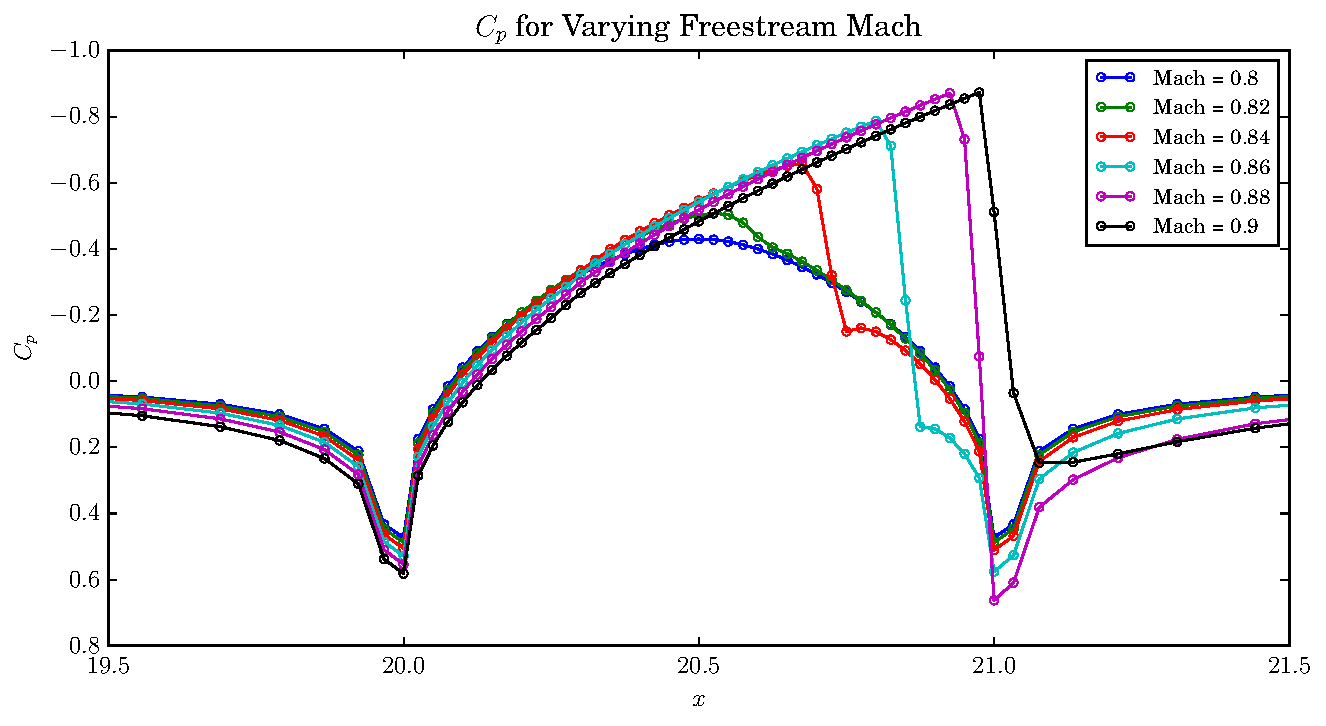
\includegraphics[width = 0.85\textwidth]{./Figures/cpsurf.pdf}
    \caption{$C_p$ Surface Distribution}
    \label{fig:cpsurf}
\end{figure}

\begin{figure}[!htbp]
\centering
\foreach \i in {80,82,84} {%
    \begin{subfigure}[p]{0.83\textwidth}
        \includegraphics[width=\linewidth]{./Figures/cpcontour_\i.pdf}
    \end{subfigure}
}
\caption{$C_p$ Contour Plots for Mach = 0.80, 0.82, 0.84}
\label{fig:cpcontour8084}
\end{figure}

\begin{figure}[!htbp]
\centering
\foreach \i in {86,88,90} {%
    \begin{subfigure}[p]{0.83\textwidth}
        \includegraphics[width=\linewidth]{./Figures/cpcontour_\i.pdf}
    \end{subfigure}
}
\caption{$C_p$ Contour Plots for Mach = 0.86, 0.88, 0.90}
\label{fig:cpcontour8690}
\end{figure}

\clearpage

\section*{Grid Study}

The coefficient of pressure $C_p$ for the coarse, medium and fine grid is plotted in Figure \ref{fig:q3cpsurf}.
The shock location minimally moves upstream as the grid is refined.
From the location of the points on the shock, the reason could be simply because the coarse grid does not have enough points on the airfoil to accurately represent the small recovery.
The pressure recovery is however seen in the contour plot from the previous section on the coarse grid.

\begin{figure}[!htbp]
    \centering
    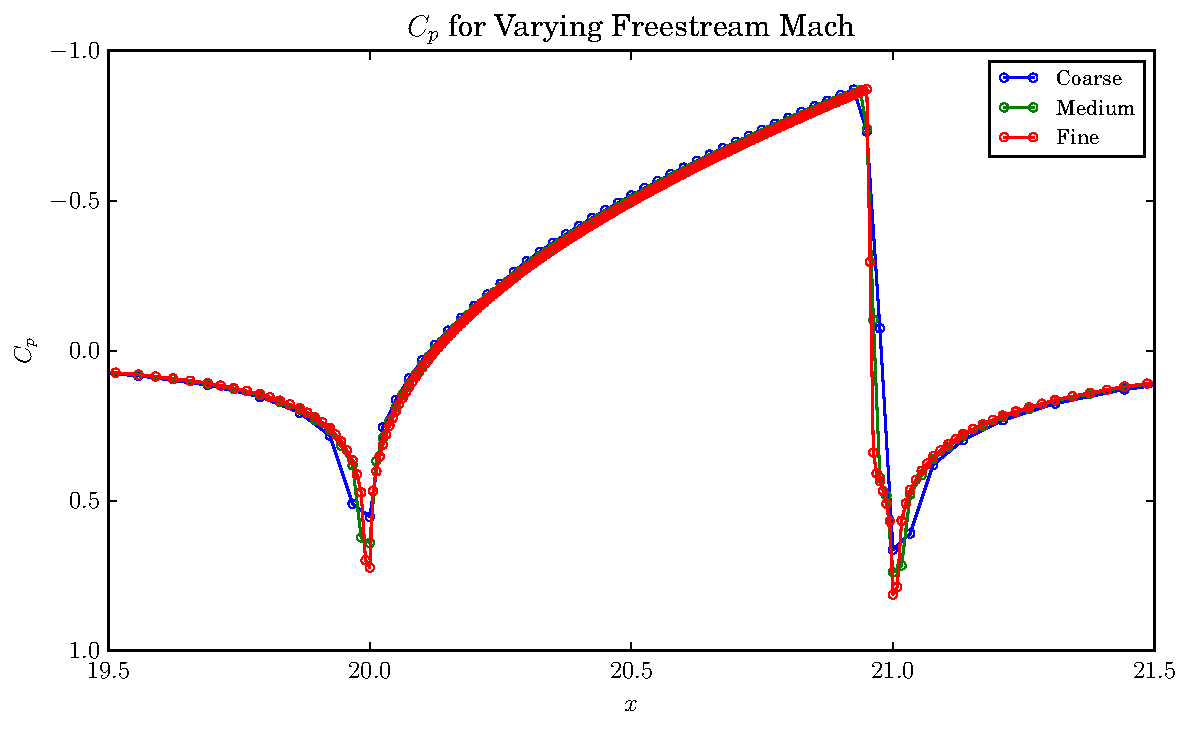
\includegraphics[width=\linewidth]{./Figures/q3cpsurf.pdf}
    \caption{$C_p$ Surface Distribution for Different Grid Sizes}
    \label{fig:q3cpsurf}
\end{figure}

\clearpage
\section*{Solvers}

This section compares the Gauss Seidel (GS) method and the line-implicit Gauss-Seidel (LGS) method.
The residual is plotted against CPU time and number of iterations Figure \ref{fig:q4time} and \ref{fig:q4res}.
The LGS method requires approximately two-thirds of the iterations of GS method to converge to 5\textsc{E-}15.
However, the lower number of iterations is offset by the higher CPU time per iteration.

The earlier iterations converge much quicker for the LGS method until approximately 1\textsc{E-}9.
Then, each step afterwards does not improve the solution enough to offset the high CPU time cost.
The convergence to machine precision ends up between fairly equal in terms of CPU time if machine precision is required.
If a lower tolerance is acceptable, LGS will be quicker to converge.


\begin{figure}[!htbp]
    \centering
    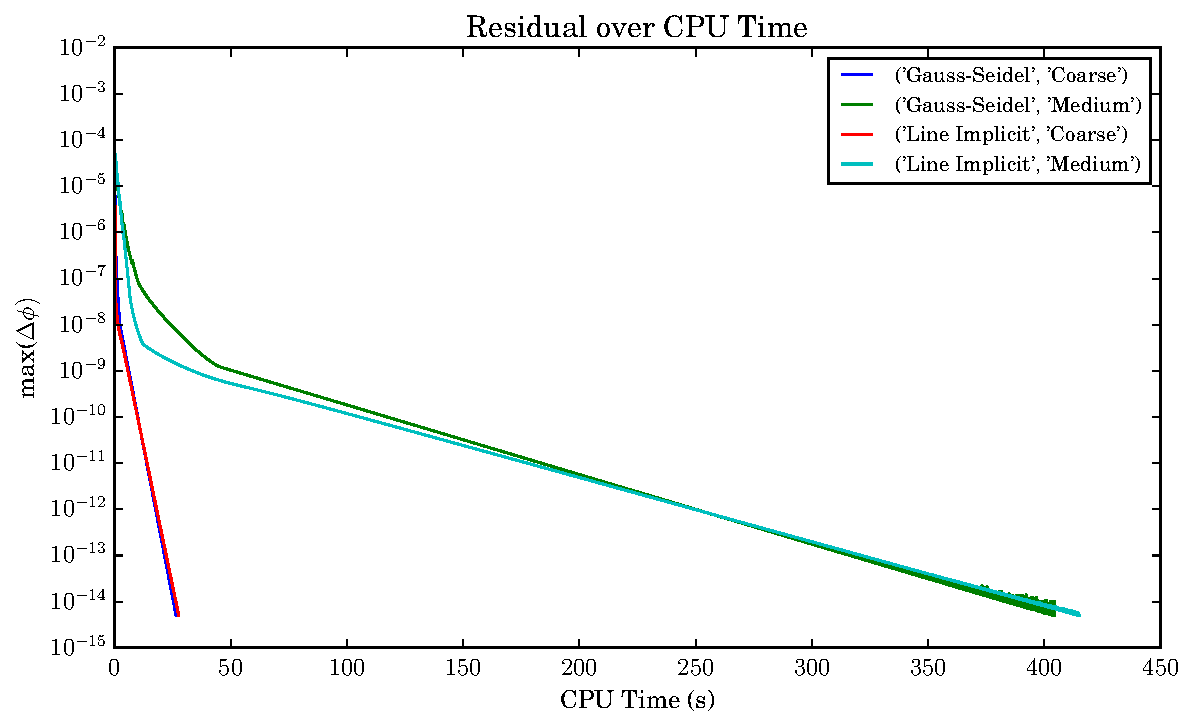
\includegraphics[width=\linewidth]{./Figures/q4time.pdf}
    \caption{Convergence over CPU Time}
    \label{fig:q4time}
\end{figure}

\begin{figure}[!htbp]
    \centering
    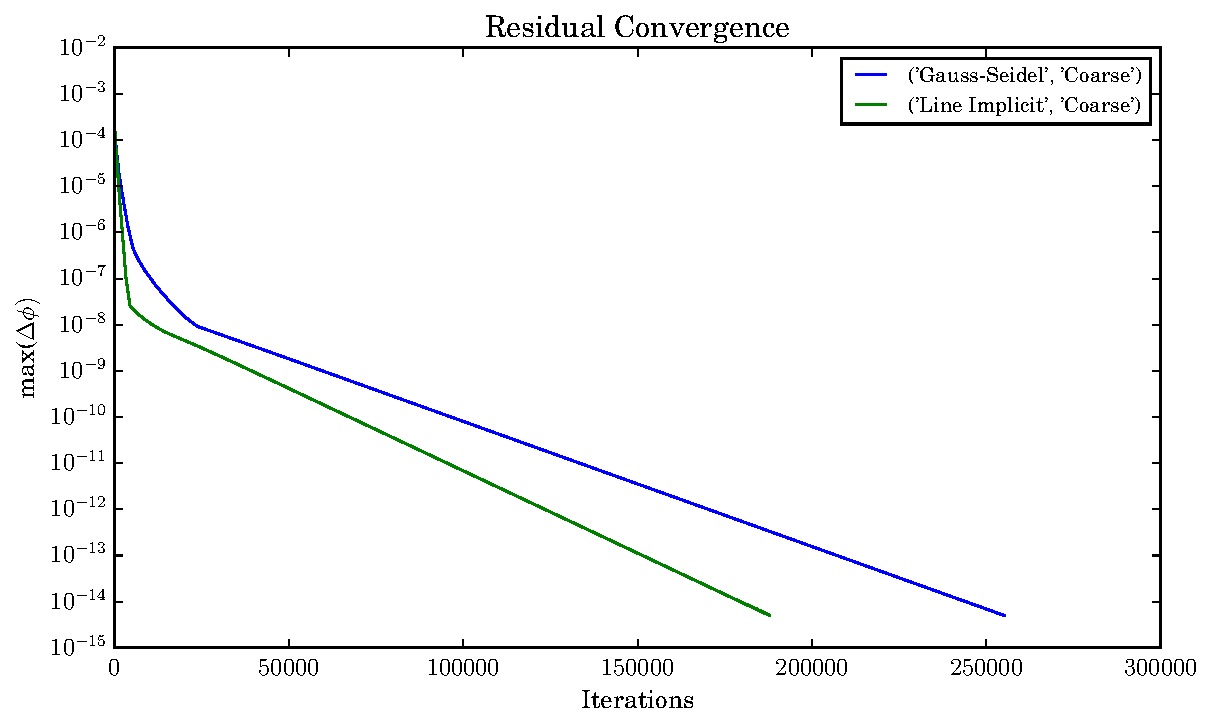
\includegraphics[width=\linewidth]{./Figures/q4res.pdf}
    \caption{Convergence over the Iterations}
    \label{fig:q4res}
\end{figure}

\clearpage
\section*{Codes}

Code has been written in FORTRAN. Default arithmetic operations are in double precision and optimization level -O3.

All codes are available on my GitHub:

\url{https://github.com/dougshidong/mech539/tree/master/a3}

\end{document}
